% !TeX TS-program = xelatex

\documentclass[dvipsnames]{beamer}
\usetheme{metropolis}

\usepackage{multicol}

\usepackage{xecolor}
\usepackage{amsmath}
% \usefonttheme[onlymath]{serif} % change the math font

\usepackage{ragged2e}
\usepackage{tabularx}
\usepackage{booktabs}
\usepackage[style=numeric,sorting=ynt]{biblatex}
\addbibresource{references.bib}
\usepackage[localise]{xepersian}

\settextfont[
	Path = fonts/,
	UprightFont = *-Regular,
	BoldFont = *-Bold,
	ItalicFont = *-Variable
]{Vazir}
\setlatintextfont[
	Path = fonts/,
	UprightFont = *-Regular,
	BoldFont = *-Bold,
	ItalicFont = *-Italic
]{Neuton}

% ---------------------------------------------------------------------------------
% Colors
% ---------------------------------------------------------------------------------
\definecolor{نارنجی}{rgb}{1.0, 0.31, 0.0}

% To force beamer use numbering in captions
\setbeamertemplate{caption}[numbered]{}% Number float-like environments

\setbeamertemplate{footline}[frame number]
\setbeamertemplate{section in toc}[circle]
\setbeamertemplate{blocks}[rounded][shadow=true]
\setbeamercolor{block title}{bg=orange}
\setbeamercolor{block body}{bg=lightgray}
\setbeamercolor{headline}{bg=orange}
\setbeamersize{text margin left=1cm,text margin right=1cm}
\setbeamertemplate{frametitle continuation}{\insertcontinuationcount}

\setbeamertemplate{headline}
{
	\begin{beamercolorbox}{section in head/foot}
		\vspace{2pt}\insertnavigation{\paperwidth}\vspace{2pt}
	\end{beamercolorbox}
}

\setbeamertemplate{footline}
{%
	\leavevmode%
	\hbox{%
		\begin{beamercolorbox}[wd=.333333\paperwidth,ht=2.25ex,dp=1ex,center]{author in head/foot}%
			\usebeamerfont{author in head/foot}\insertshortauthor%
		\end{beamercolorbox}%
		\begin{beamercolorbox}[wd=.333333\paperwidth,ht=2.25ex,dp=1ex,center]{title in head/foot}%
			\usebeamerfont{title in head/foot}\insertshorttitle%
		\end{beamercolorbox}%
		\begin{beamercolorbox}[wd=.333333\paperwidth,ht=2.25ex,dp=1ex,right]{date in head/foot}%
			\usebeamerfont{date in head/foot}\insertsection\hspace*{2em}
			\insertframenumber~ از \inserttotalframenumber{} \hspace*{2ex}%
		\end{beamercolorbox}
	}%
}

% ---------------------------------------------------------------------------------
\title{ارزیابی انتها به انتها شبکه \متن‌لاتین{LoRaWAN}}
\subtitle{}
\author{پرهام الوانی}
\institute{%
	دانشکده مهندسی کامپیوتر\\
	دکتر بهادر بخشی و دکتر مهدی راستی
}
\date{\today}
\titlegraphic{\vspace{4.5cm}\flushleft
\includegraphics[height=50pt]{images/logo}}

\setbeamertemplate{title}{%
	\linespread{1.0}%
	\inserttitle%
	\par%
	\vspace*{0.5em}
}
\setbeamertemplate{subtitle}{%
	\insertsubtitle%
	\par%
	\vspace*{0.5em}
}

\AtBeginSection[]
{%
	\begin{frame}{فهرست}
	  \RaggedLeft
	  \tableofcontents[currentsection]
	\end{frame}
	\begin{frame}
		\begin{center}
			\insertsectionnumber. \insertsection%
		\end{center}
		\usebeamertemplate*{title separator}
	\end{frame}
}

\begin{document}

\begin{persian}

	% ------------------------------------------
	% Title frame (0)
	% ------------------------------------------
	{%
		\setbeamertemplate{footline}{}
		\begin{frame}
		  \titlepage%
		\end{frame}
	}

	% -------------------------------------------------------------------------------
	\begin{frame}{فهرست}
	  \RaggedLeft
	  \tableofcontents[pausesections]
	\end{frame}

	% -------------------------------------------------------------------------------
	\قسمت{مقدمه}

	\begin{frame}{اینرتنت اشیا}
	  \تنظیم‌ازوسط
	  \درج‌تصویر[width=\textwidth]{./images/iot-growth.jpg}
	\end{frame}

	\begin{frame}{شبکه‌های توان پایین با برد بلند}
		\شروع{فقرات}
		\فقره عدم همخوانی تکنولوژی‌های حاضر شبکه‌های حسگر بی‌سیم با گسترش روزافزون اینترنت اشیا
		\شروع{فقرات}
		\فقره کاهش هزینه‌های هر واحد
		\فقره گسترده‌تر کردن پوشش شبکه
		\فقره کاهش توان مصرفی نودهای در لبه
		\فقره شبکه‌های گسترش‌پذیر
		\پایان{فقرات}
		\pause
		\فقره \متن‌لاتین{LPWAN} یا \متن‌لاتین{Low-Power Wide Area Network}
		\پایان{فقرات}
	\end{frame}

	\begin{frame}{شبکه‌های توان پایین با برد بلند}
	  \شروع{فقرات}
	  \فقره مهم‌ترین شبکه‌های توان پایین با برد بلند:
	  \شروع{فقرات}
	  \فقره \متن‌لاتین{LoRa}
	  \فقره \متن‌لاتین{Sigfox}
	  \فقره \متن‌لاتین{NB-IoT}
	  \پایان{فقرات}
	  \pause
	  \فقره شاخصه‌های شبکه‌های \متن‌لاتین{LoRa}
	  \شروع{فقرات}
	  \فقره استفاده از باند فرکانسی بدون مجوز
	  \فقره امکان راه‌اندازی شبکه توسط اشخاص ثالث
	  \پایان{فقرات}
	  \pause
	  \فقره پرداختن پژوهش‌های زیادی در این سال‌ها به شبکه‌های \متن‌لاتین{LoRa}
	  \فقره \متن‌لاتین{LoRa} بیشترین تکنولوژی استفاده شده
	  \پایان{فقرات}
	\end{frame}

	\begin{frame}{شبکه‌های \متن‌لاتین{LoRaWAN}}
	  \شروع{فقرات}
	  \فقره لایه پیوند داده بر پایه لایه فیزیکی \متن‌لاتین{LoRa}
	  \فقره استاندارد رایگان بر خلاف \متن‌لاتین{LoRa}
	  \فقره عدم وجود ارتباط میان دروازه‌ها و گره‌ها وجود ندارد
	  \فقره داده‌ی ارسالی توسط هر گره می‌تواند به وسیله‌ی یک یا چند دروازه دریافت شود.
	  \فقره دروازه‌ها وظیفه ارسال ترافیک گره‌های \متن‌لاتین{LoRa} به سرور شبکه و برعکس را دارا هستند.
	  \فقره عملیات‌هایی از جمله احراز هویت، شناسایی و حذف بسته‌های تکراری توسط سرور شبکه صورت می‌پذیرد.
	  \پایان{فقرات}
	\end{frame}

	\begin{frame}
		\begin{figure}
		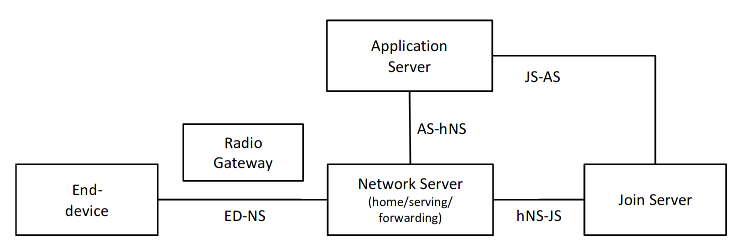
\includegraphics[width=\textwidth]{./images/nrm-home.png}
		\centering
		\caption{مدل مرجع شبکه \متن‌لاتین{LoRaWAN} - شبکه‌ی خانگی}
		\end{figure}
	\end{frame}

	\section{کارهای مرتبط}

	\begin{frame}{ارزیابی شبکه دسترسی}
		\fontsize{5pt}{6pt}\selectfont
		\begin{tabularx}{\textwidth}{|*{13}{X|}}
			\toprule
			مرجع &
			جابجایی &
			پوشش‌دهی &
			شبکه &
			لایه انتقال &
			لایه اپلیکشن &
			اندازه بسته &
			نرخ کدگذاری &
			تاخیر &
			محیط &
			\متن‌لاتین{LoRa Mesh} &
			توان مصرفی &
			شبیه‌سازی \\
			\midrule
			\cite{sensors-18-00772-v3} &
			سیار &
			گزارش شده &
			\متن‌لاتین{LoRa} &
			ندارد &
			ندارد &
			گزارش شده &
			گزارش شده &
			گزارش نشده &
			باز &
			ندارد &
			گزارش نشده &
			واقعی / \متن‌لاتین{cloudRF} \\
			\midrule
			\cite{sensors-19-00007} &
			ثابت &
			گزارش شده &
			\متن‌لاتین{NB-IoT} &
			\متن‌لاتین{TCP / UDP} &
			\متن‌لاتین{MQTT / CoAP} &
			گزارش شده &
			گزارش نشده &
			گزارش شده &
			باز &
			ندارد &
			گزارش نشده &
			\متن‌لاتین{Ericsson inter. sim.} \\
			\midrule
			\cite{sensors-20-03061-v2} &
			ثابت &
			گزارش شده &
			\متن‌لاتین{LoRa} &
			ندارد &
			ندارد &
			گزارش شده &
			گزارش شده &
			گزارش شده &
			باز / بسته &
			ندارد &
			گزارش نشده &
			\متن‌لاتین{ns-3} \\
			\midrule
			\cite{sensors-20-00280-v2} &
			ثابت &
			گزارش شده &
			\متن‌لاتین{LoRa} &
			\متن‌لاتین{UDP ov IPv6} &
			\متن‌لاتین{CoAP} &
			گزارش شده &
			گزارش شده &
			گزارش شده &
			باز / بسته &
			ندارد &
			گزارش شده &
			واقعی \\
			\midrule
			\cite{sensors-20-06721} &
			ثابت &
			گزارش شده &
			\متن‌لاتین{LoRa} &
			ندارد &
			ندارد &
			گزارش شده &
			گزارش شده &
			گزارش شده &
			بسته &
			ندارد &
			گزارش شده &
			واقعی \\
			\midrule
			\cite{SanchezIborra2020} &
			متحرک &
			گزارش شده &
			\متن‌لاتین{LoRa \ NB-IoT} &
			\متن‌لاتین{UDP/TCP ov IPv6} &
			\متن‌لاتین{CoAP / ReST} &
			گزارش شده &
			گزارش شده &
			گزارش شده &
			باز &
			ندارد &
			گزارش شده &
			واقعی \\
			\midrule
			\cite{Lee2018} &
			ثابت &
			گزارش شده &
			\متن‌لاتین{LoRa} &
			ندارد &
			ندارد &
			گزارش نشده &
			گزارش شده &
			گزارش شده &
			باز / بسته &
			دارد &
			گزارش نشده &
			واقعی \\
			\midrule
			\cite{Marahatta2021} &
			ثابت &
			گزارش شده &
			\متن‌لاتین{LoRa} &
			ندارد &
			ندارد &
			گزارش شده &
			گزارش شده &
			گزارش شده &
			باز / بسته &
			دارد &
			گزارش نشده &
			\متن‌لاتین{ns-2} \\
			\bottomrule
		\end{tabularx}
	\end{frame}

	\begin{frame}{ارزیابی شبکه دسترسی}
	  \شروع{فقرات}
	  \فقره پژوهشگران \مرجع{sensors-20-06721} تجربه بیش از دو سال نگهداری از شبکه‌ی سنسورهای فضای بسته دانشگاه \متن‌لاتین{oulu} کشور فلاند مبتنی بر \متن‌لاتین{LoRaWAN} در این پژوهش مرور می‌کنند.
	  \فقره یکی از موارد مهمی که در این پژوهش به آن اشاره می‌شود، از دست رفتن بسته‌ها به جز در شبکه‌ی دسترسی و
	  شبکه میان میان سرور شبکه و سرور پلتفرم است.
	  \فقره این پژوهش به بررسی بیشتر این موضوع نپرداخته است و دلیلی ارائه نمی‌دهد.
	  \پایان{فقرات}
	\end{frame}

	\begin{frame}{تاخیر انتها به انتها}
	  \شروع{فقرات}
	  \فقره پژوهش \مرجع{FernandesCarvalho2019}
	  \شروع{فقرات}
	  \فقره ارائه روش ارزیابی تاخیر \متن‌لاتین{uplink} در استقرارهای \متن‌لاتین{LoRaWAN}
	  \پایان{فقرات}
	  \فقره پژوهش \مرجع{Carvalho2019}
	  \شروع{فقرات}
	  \فقره ارزیابی تاخیر ناشی از زیرساخت \متن‌لاتین{LoRaWAN} از دروازه تا سرور شبکه
	  \فقره بیشترین تاخیر در سرور شبکه
	  \پایان{فقرات}
	  \فقره پژوهش \مرجع{Potsch2019}
	  \شروع{فقرات}
	  \فقره ارزیابی استقرار محلی و ابری زیرساخت شبکه‌ی \متن‌لاتین{LoRaWAN} از جهت تاخیر بسته از گره تا دریافت کامل بسته در برنامه کاربردی
	  \پایان{فقرات}
	  \پایان{فقرات}
	\end{frame}

	\begin{frame}{پروتکل‌های وب}
	  \شروع{فقرات}
	  \فقره پژوهش \مرجع{sensors-20-00280-v2}
	  \شروع{فقرات}
	  \فقره پیاده‌سازی الگوریتم \متن‌لاتین{Static Context Header Compression (SCHC)} برای \متن‌لاتین{IPv6}
	  \فقره ارزیابی انتقال پروتکل \متن‌لاتین{CoAP} بر بستر \متن‌لاتین{UDP} با استفاده از این الگوریتم
	  \پایان{فقرات}
	  \پایان{فقرات}
	\end{frame}

	\begin{frame}{شکاف تحقیقاتی}
	  \شروع{فقرات}
	  \فقره نپرداختن پژوهش‌ها به معماری انتها به انتها \متن‌لاتین{LoRaWAN}
	  \فقره وجود بیشتر پردازش‌ها را در سمت شبکه هسته \متن‌لاتین{LoRaWAN}
	  \فقره معماری \متن‌لاتین{LoRaWAN} به صورت انتها به انتها و با چگالی بالا مورد ارزیابی قرار نگرفته است.
	  \فقره پروتکل‌هایی مانند \متن‌لاتین{IPv6} در شبکه‌های \متن‌لاتین{LoRaWAN} به صورت انتها به انتها مورد ارزیابی قرار نگرفته‌اند.
	  \پایان{فقرات}
	\end{frame}

	\begin{frame}{شکاف تحقیقاتی}
		\شروع{فقرات}
		\فقره همانطور که بیان شد بیشتر پژوهش‌ها بر روی ارزیابی شبکه‌ی دسترسی بی‌سیم تمرکز کرده‌اند.
		\فقره دیده نشده تاثیر پارامترهایی مانند نرخ ارسال، تعداد اشیا به صورت انتها به انتها
		\فقره دیده نشدن تاثیر پارامترهایی مانند ساختار داده‌ای و کدگذاری داده در ارتباط میان گره‌ها و برنامه‌های کاربردی اینترنت اشیا
		\پایان{فقرات}
	\end{frame}

	\قسمت{بیان مسائل و رویکرد حل مساله}

	\begin{frame}{ارزیابی شبکه دسترسی در شبکه \متن‌لاتین{LoRaWAN} از دروازه تا سرور شبکه و سرور اپلیکیشن}
		\شروع{فقرات}
		\فقره ارزیابی شبکه هسته مبتنی بر \متن‌لاتین{IP} در معماری \متن‌لاتین{LoRaWAN}
		\فقره معیارهای کارایی:
		\شروع{فقرات}
		\فقره نرخ دریافت صحیح بسته
		\فقره تاخیر
		\فقره بهره‌وری
		\پایان{فقرات}
		\پایان{فقرات}
	\end{frame}

	\begin{frame}{پارامترهای موثر}
	  \شروع{فقرات}
	  \فقره تاخیر:

	  \شروع{فقرات}
	  \فقره تاخیر ارسال از دروازه بر بستر \متن‌لاتین{IP}
	  \فقره تاخیر صف و پردازش در شبکه \متن‌لاتین{IP} میان دروازه و سرور شبکه
	  \فقره تاخیر پردازش در سرور شبکه
	  \فقره تاخیر صف و پردازش در شبکه \متن‌لاتین{IP} میان سرور شبکه و سرور اپلیکیشن
	  \فقره تاخیر پردازش در سرور اپلیکیشن
	  \فقره تاخیر صف و پردازش در شبکه \متن‌لاتین{IP} میان سرور اپلیکیشن و پلتفرم
	  \پایان{فقرات}

	  نرخ از دست رفت بسته

	  \شروع{فقرات}
	  \فقره از دست رفت بسته در شبکه \متن‌لاتین{IP} میان دروازه و سرور شبکه
	  \فقره از دست رفت بسته در سرور شبکه
	  \فقره از دست رفت بسته در شبکه \متن‌لاتین{IP} میان سرور شبکه و سرور اپلیکیشن
	  \فقره از دست رفت بسته در سرور اپلیکیشن
	  \فقره از دست رفت بسته در شبکه \متن‌لاتین{IP} میان سرور اپلیکیشن و پلتفرم
	  \پایان{فقرات}

	  \پایان{فقرات}
	\end{frame}

	\begin{frame}{پارامترهای موثر}
	  \شروع{فقرات}
	  \فقره بهره‌وری:

	  \شروع{فقرات}
	  \فقره بهره‌وری پروتکل ارتباطی شبکه میان دروازه و سرور شبکه
	  \فقره بهره‌وری پروتکل ارتباطی شبکه میان سرور شبکه و سرور اپلیکیشن
	  \فقره بهره‌وری پروتکل ارتباطی شبکه میان سرور اپلیکیشن و پلتفرم
	  \پایان{فقرات}

	  \پایان{فقرات}
	\end{frame}

	\begin{frame}{ارزیابی لایه کاربرد شبکه \متن‌لاتین{LoRaWAN} از گره تا اپلیکیشن}
	  \شروع{فقرات}
	  \فقره ارزیابی تاثیر پروتکل‌هایی مانند \متن‌لاتین{IPv6} به صورت انتها به انتها
	  \پایان{فقرات}
	\end{frame}

	\begin{frame}{پارامترهای موثر}
	  \شروع{فقرات}
	  \فقره تاخیر:

	  \شروع{فقرات}
	  \فقره تاخیر استفاده از \متن‌لاتین{IPv6} و \متن‌لاتین{SCHC}
	  \فقره تاخیر کدگذاری داده در گره
	  \فقره تاخیر کدگذاری داده در پلتفرم
	  \فقره تاخیر تجزیه کردن داده‌ها در پلتفرم
	  \پایان{فقرات}

	  \فقره نرخ از دست رفت بسته

	  \شروع{فقرات}
	  \فقره پروتکل ارتباطی
	  \پایان{فقرات}

	  \فقره بهره‌وری:

	  \شروع{فقرات}
	  \فقره بهره‌وری پروتکل ارتباطی
	  \پایان{فقرات}

	  \پایان{فقرات}
	\end{frame}

	\begin{frame}{}
	  \تنظیم‌ازوسط
	  \درج‌تصویر[width=\textwidth]{./images/e2e-iot-lorawan.png}
	\end{frame}

	\begin{frame}
	  \شروع{فقرات}
	  \فقره مدل‌های تحلیلی
	  \شروع{فقرات}
	  \فقره ارزیابی حالت میانگین با استفاده از تئوری صف
	  \فقره ارزیابی حالت‌های حدی با استفاده از \متن‌لاتین{Network Calculus}
	  \پایان{فقرات}

	  \فقره شبیه‌سازی نزدیک به واقعیت
	  \شروع{فقرات}
	  \فقره انجام شبیه‌سازی در شرایط مختلف مبتنی بر روش مونت کارلو
	  \فقره استفاده از پیاده‌سازی‌های واقعی برای اجزای معماری
	  \پایان{فقرات}

	  \فقره بهبودهای پیشنهادی
	  \شروع{فقرات}
	  \فقره نزدیک کردن مقادیر حاصل از شبیه‌سازی به مدل‌های تحلیلی
	  \فقره استفاده از پردازش لبه در راستای کاهش تاخیر و افزایش بهره‌وری
	  \فقره استفاده از الگوریتم‌های یادگیری تقویتی در مواردی مانند مشخص کردن تعداد بهینه دروازه‌ها
	  \پایان{فقرات}
	  \پایان{فقرات}
	\end{frame}

	\قسمت{شبیه‌سازی}

	\begin{frame}
	  \شروع{فقرات}
	  \فقره شبیه‌سازی مدل ساده شده از شبکه دسترسی \متن‌لاتین{LoRaWAN} از دروازه تا سرور شبکه و سرور اپلیکیشن
	  \فقره معیارهای تاخیر و نرخ از دست رفته بسته‌ها
	  \فقره ارزیابی تاثیر افزایش نرخ ارسال اشیا
	  \فقره ارزیابی تاثیر افزایش تعداد اشیا
	  \فقره ارزیابی تاثیر افزایش تعداد دروازه‌ها
	  \پایان{فقرات}
	\end{frame}

	\begin{frame}
	  \شروع{فقرات}
	  \فقره استفاده از پیاده‌سازی \متن‌لاتین{Chirpstack} برای شبکه هسته
	  \فقره ارسال داده‌ها از یک دروازه شبیه‌سازی شده با پروتکل \متن‌لاتین{MQTT} به سرور شبکه
	  \فقره ارتباط \متن‌لاتین{gRPC} میان سرور شبکه و سرور اپلیکیشن
	  \فقره دریافت داده از سرور اپلیکیشن با پروتکل \متن‌لاتین{MQTT}
	  \فقره استفاده از کدگذاری \متن‌لاتین{CBOR} برای داده‌ها
	  \پایان{فقرات}
	\end{frame}

	\begin{frame}
		\begin{figure}
		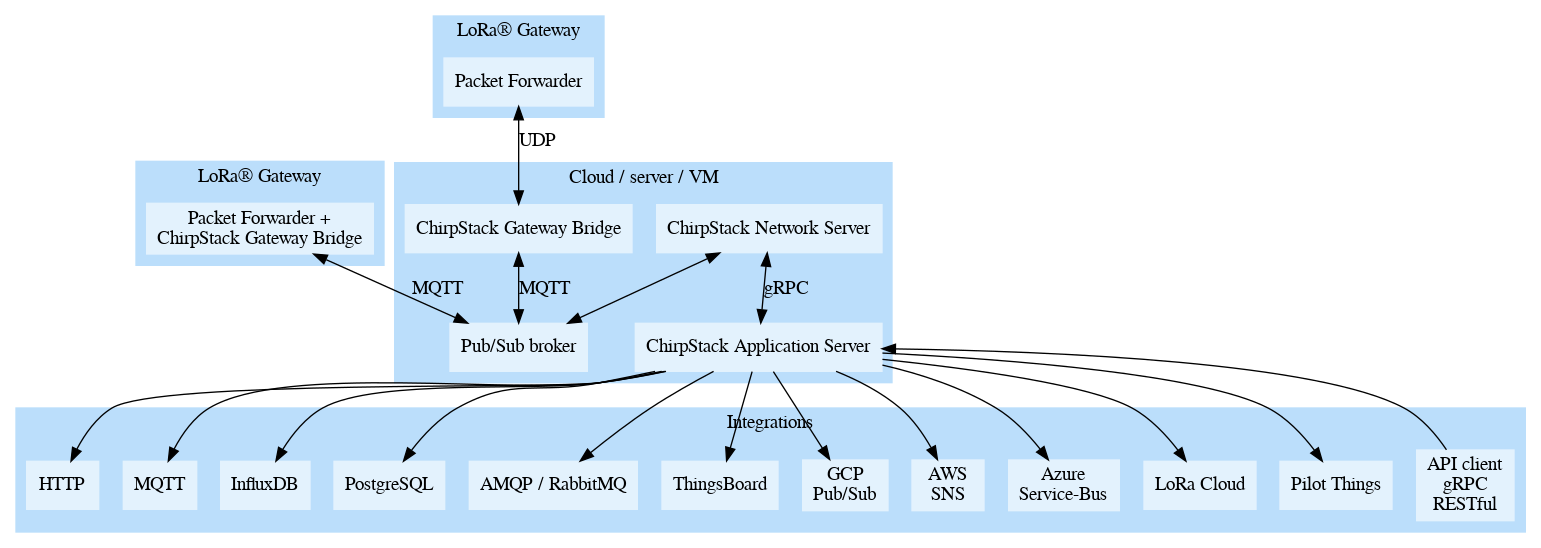
\includegraphics[width=\textwidth]{./images/chirpstack-architecture.png}
		\centering
		\caption{معماری \متن‌لاتین{LoRaWAN} سرور متن باز \متن‌لاتین{Chirpstack}}
		\end{figure}
	\end{frame}

	\begin{frame}
	  \تنظیم‌ازوسط
	  \درج‌تصویر[height=\textheight]{../proposal/simulation/s1/e7.png}
	\end{frame}

	\begin{frame}
	  \شروع{فقرات}
	  \فقره افزایش تعداد دروازه‌ها
	  \شروع{فقرات}
	  \فقره افزایش نرخ دریافت صحیح بسته‌ها در شبکه دسترسی بی‌سیم
	  \فقره کاهش نرخ دریافت صحیح بسته‌ها در شبکه هسته
	  \پایان{فقرات}
	  \پایان{فقرات}
	\end{frame}

	\قسمت{جمع‌بندی}

	\begin{frame}{گام‌های آینده}
	  \شروع{فقرات}
	  \فقره ارائه یک سیستم ارزیابی نزدیک به واقعیت در جهت ارزیابی استقرارهای مختلف \متن‌لاتین{LoRaWAN}
	  \فقره ارائه مدل‌های تحلیلی
	  \فقره ارائه و ارزیابی بهبودها
	  \پایان{فقرات}
	\end{frame}

	\begin{frame}{گام‌های آینده}
	  \تنظیم‌ازوسط
	  \درج‌تصویر[width=\textwidth]{./images/gantt.png}
	\end{frame}

	% -------------------------------------------------------------------------------
	\begin{frame}[allowframebreaks]{مراجع}
		\begin{latin}
			\printbibliography[title=مراجع]
		\end{latin}
	\end{frame}

\end{persian}
\end{document}
